\documentclass[times,a4paper,titlepage,12pt]{article}

\usepackage{anysize}
\marginsize{30mm}{20mm}{30mm}{20mm}

\usepackage{times}
\usepackage[brazil]{babel}
\usepackage[latin1]{inputenc}
\usepackage[T1]{fontenc}
\usepackage{cite}
\usepackage{epsfig}
\usepackage{graphicx}
\usepackage{booktabs}
\usepackage{fancyhdr}
\usepackage{url}
\usepackage{enumerate}
\usepackage{amsmath}
\usepackage[alf]{abntex2cite}
\setcounter{tocdepth}{2}
\linespread{1.1}

% Para colocar a numera��o das p�ginas do lado direito inferior
\fancyhf{} % clear all header and footer fields
\fancyfoot[R]{\footnotesize \thepage\ }
\renewcommand{\headrulewidth}{0pt}
\renewcommand{\footrulewidth}{0pt}
\addtolength{\headwidth}{\marginparsep}\addtolength{\headwidth}{\marginparwidth}\headwidth
= \textwidth
%%%%%%%%%%%%%%%%%%%%%%%%%%%%%%%%%%%%%%%%%%%%%%%%%%%%%%%%%%%%%%


\hyphenation{}

\begin{document}
\pagestyle{empty}

\begin{figure}
\centering
  
\includegraphics[width=0.15\textwidth]{./img/uea}
  %\includegraphics[width=0.15\textwidth]{./fig/est}\\
\end{figure}


\begin{center}
\LARGE{
Universidade do Estado do Amazonas\\
Escola Superior de Tecnologia}\\
\end{center}

\vspace{1.5cm}


\begin{center}
\Large{Programa de Apoio � Inicia��o Cient�fica}\\
\large{(PAIC/FAPEAM/UEA)}\\
\end{center}

\vspace{1.5cm}

\begin{center}
\Large{\textbf{Previs�o da Cota do Rio Negro\\ Utilizando Redes Neurais Artificiais}}\\
\large{(T�tulo do Projeto)}
\end{center}

\vspace{1cm}


\begin{center}
\textbf{Janderson do Nascimento Lira}\\
\texttt{janderson.nlira@gmail.com}\\
(Aluno)
\end{center}

\vspace{1cm}

\begin{center}
\textbf{Profa. Dra. Ello� Barreto Guedes da Costa}\\
\texttt{elloa.uea@gmail.com}\\
(Orientadora)
\end{center}



\vspace{2cm}

\begin{center}
{\small Manaus -- Amazonas -- Brasil \\
\today
}
\end{center}

\newpage
\cleardoublepage


\pagestyle{fancy}

\tableofcontents
\newpage

\section{Introdu��o}
Para lidar com problemas que n�o se conhece uma solu��o anal�tica, uma estrat�gia amplamente utilizada � usar dados sobre esse problema na tentativa de elaborar uma solu��o emp�rica. Esta abordagem � amplamente utilizada por muitas �reas da Ci�ncia, Engenharia, Economia e outras �reas do conhecimento \cite{Mostafa:LearningData}.

O \emph{Aprendizado de M�quina} (AM) � uma sub�rea da Intelig�ncia Artificial que lida com a elabora��o de solu��es emp�ricas com a utiliza��o de modelos e m�todos computacionais que aprendem a partir de dados.  Neste contexto, o termo ``aprender'' adquire uma conota��o de aumentar a performance sobre uma tarefa em rela��o � um momento anterior \cite{Witten:DataMining}.

O AM utiliza-se de teorias estat�sticas na elabora��o destes modelos e m�todos, pois a sua principal tarefa consiste na elabora��o de infer�ncias a partir de amostras. Al�m da Estat�stica, a Ci�ncia da Computa��o tamb�m possui um papel relevante no Aprendizado de M�quina, pois � necess�rio construir algoritmos eficientes para diversas tarefas, tais como para lidar com um grande volume de dados, para realizar o treinamento, para infer�ncia, etc \cite{Alpayadin:MachineLearning}.

Em rela��o aos tipos de tarefas em que se pode aprender com os dados, h� duas classifica��es poss�veis: as \emph{tarefas de previs�o} e as \emph{tarefas de classifica��o}. Nas tarefas de previs�o, a meta � encontrar um modelo a partir dos dados de treinamento que possa ser utilizado para prever um valor que caracterize um novo exemplo, com base nos valores de seus atributos de entrada. No caso das tarefas de classifica��o, a meta � explorar ou descrever um conjunto de dados \cite{Lorena:Livro}.

Os modelos e m�todos do AM utilizados nas tarefas de natureza preditiva seguem o \emph{paradigma de aprendizado supervisionado}. De acordo com este paradigma, o conjunto de dados cont�m exemplos expl�citos da sa�da correta para determinadas entradas. No caso das tarefas de classifica��o, os modelos e m�todos seguem o \emph{paradigma de aprendizado n�o supervisionado}, no qual o objetivo �  detectar espontaneamente padr�es ou alguma estrutura a partir da pr�pria entrada \cite{Mostafa:LearningData}.

O ferramental de modelos e m�todos utilizados pela AM � extenso. Para as tarefas de previs�o, destacam-se as �rvores de decis�o, as redes neurais, as m�quinas de vetores de suporte, os algoritmos gen�ticos e as redes Bayesianas. No caso das tarefas de classifica��o, um vasto conjunto de t�cnicas de agrupamento encontra-se dispon�vel na literatura \cite{Haykin:NeuralNetworksBook}.

Existem v�rias aplica��es bem-sucedidas de t�cnicas de Aprendizado de M�quina na solu��o de problemas reais. Algumas das �reas beneficiadas com estas aplica��es s�o: Agropecu�ria, Bioinform�tica, Ecologia e Meio Ambiente, Energia, Finan�as, Rob�tica, Medicina, dentre diversas outras \cite{Lorena:Livro}.

No escopo deste projeto de inicia��o cient�fica, pretende-se considerar a utiliza��o de uma das t�cnicas da Aprendizagem de M�quina, as Redes Neurais Artificiais, para lidar com o problema da previs�o da cota do Rio Negro. Para tanto, uma vis�o geral do contexto deste problema ser� apresentada a seguir.

A Bacia Amaz�nica � a maior bacia hidrogr�fica do mundo, com uma �rea de aproximadamente cinco milh�es de quil�metros quadrados. De toda a �rea, cerca de $60$\% localiza-se em territ�rio brasileiro, compreendendo tr�s milh�es, oitocentos e cinquenta mil quil�metros quadrados, que representam $45$\% do territ�rio nacional \cite{Goncalves:Amazonia}. Os principais rios dessa bacia s�o: Rio Amazonas, Rio Negro, Rio Solim�es, Rio Xingu, Rio Madeira, Rio Tocantins, Rio Japur�, Rio Juru�, Rio Purus, Rio Tapaj�s, Rio Branco, Rio Jari e Rio Trombetas. Um mapa que enfatiza a parte brasileira da Bacia Amaz�nia e os rios mencionados pode ser visto na Figura \ref{img:baciaAmazonica}.


\begin{figure}[h!]
\centering
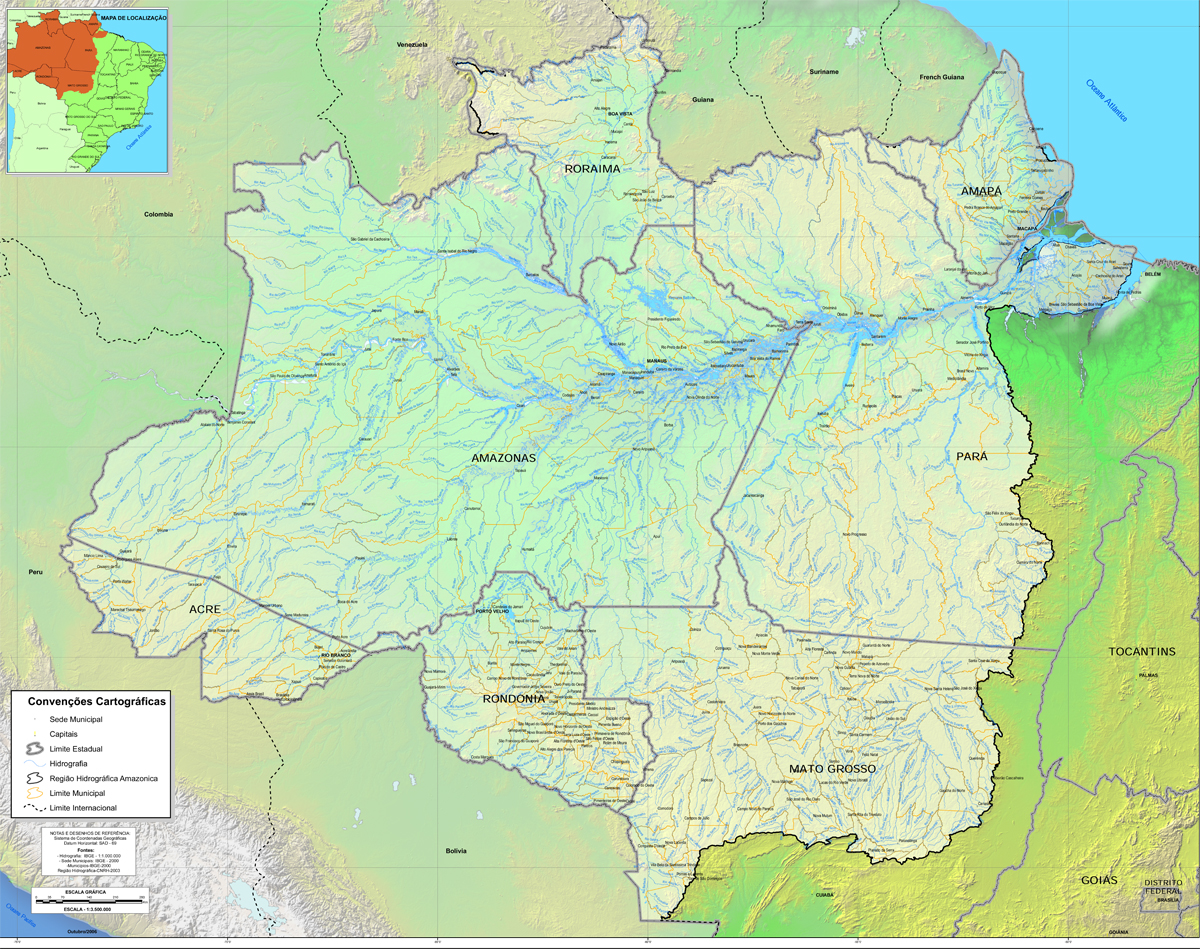
\includegraphics[width=0.6\textwidth]{./img/baciaAmazonica}
\caption{Parte Brasileira da Bacia Amaz�nica. Fonte: Ag�ncia Nacional de �guas}
\label{img:baciaAmazonica}
\end{figure}

A Bacia Amaz�nica possui um papel importante no transporte hidrovi�rio no estado do Amazonas. Em um contexto hist�rio, a malha fluvial desta bacia foi determinante na forma de ocupa��o e determinou a localiza��o da grande maioria das cidades que se afixaram nas margens dos rios \cite{Kuwahara:Navegabilidade}. Atualmente, esta bacia possui um total de $22$ mil quil�metros naveg�veis, sendo utilizados para o transporte de pessoas e mercadorias na regi�o \cite{ANTAQ:RiosGeral}.

O Rio Negro, em particular, � o maior afluente da marquem esquerda do Rio Amazonas. �s suas margens localiza-se a cidade de Manaus, na qual o Porto de Manaus constitui a principal porta de entrada para o Estado do Amazonas. Este rio � naveg�vel por $720$km acima de sua foz. Sua profundidade pode variar drasticamente, especialmente no per�odo de seca, nos quais a profundidade de determinados pontos chega ao n�vel de apenas $1$ metro. No Porto de Manaus s�o efetuadas medidas di�rias da cota do Rio Negro \cite{Porto:Institucional}. Um registro de v�rias cotas hist�ricas encontra-se afixado em determinado ponto deste porto, conforme mostra a Figura \ref{img:cotas}.


\begin{figure}[h!]
\centering
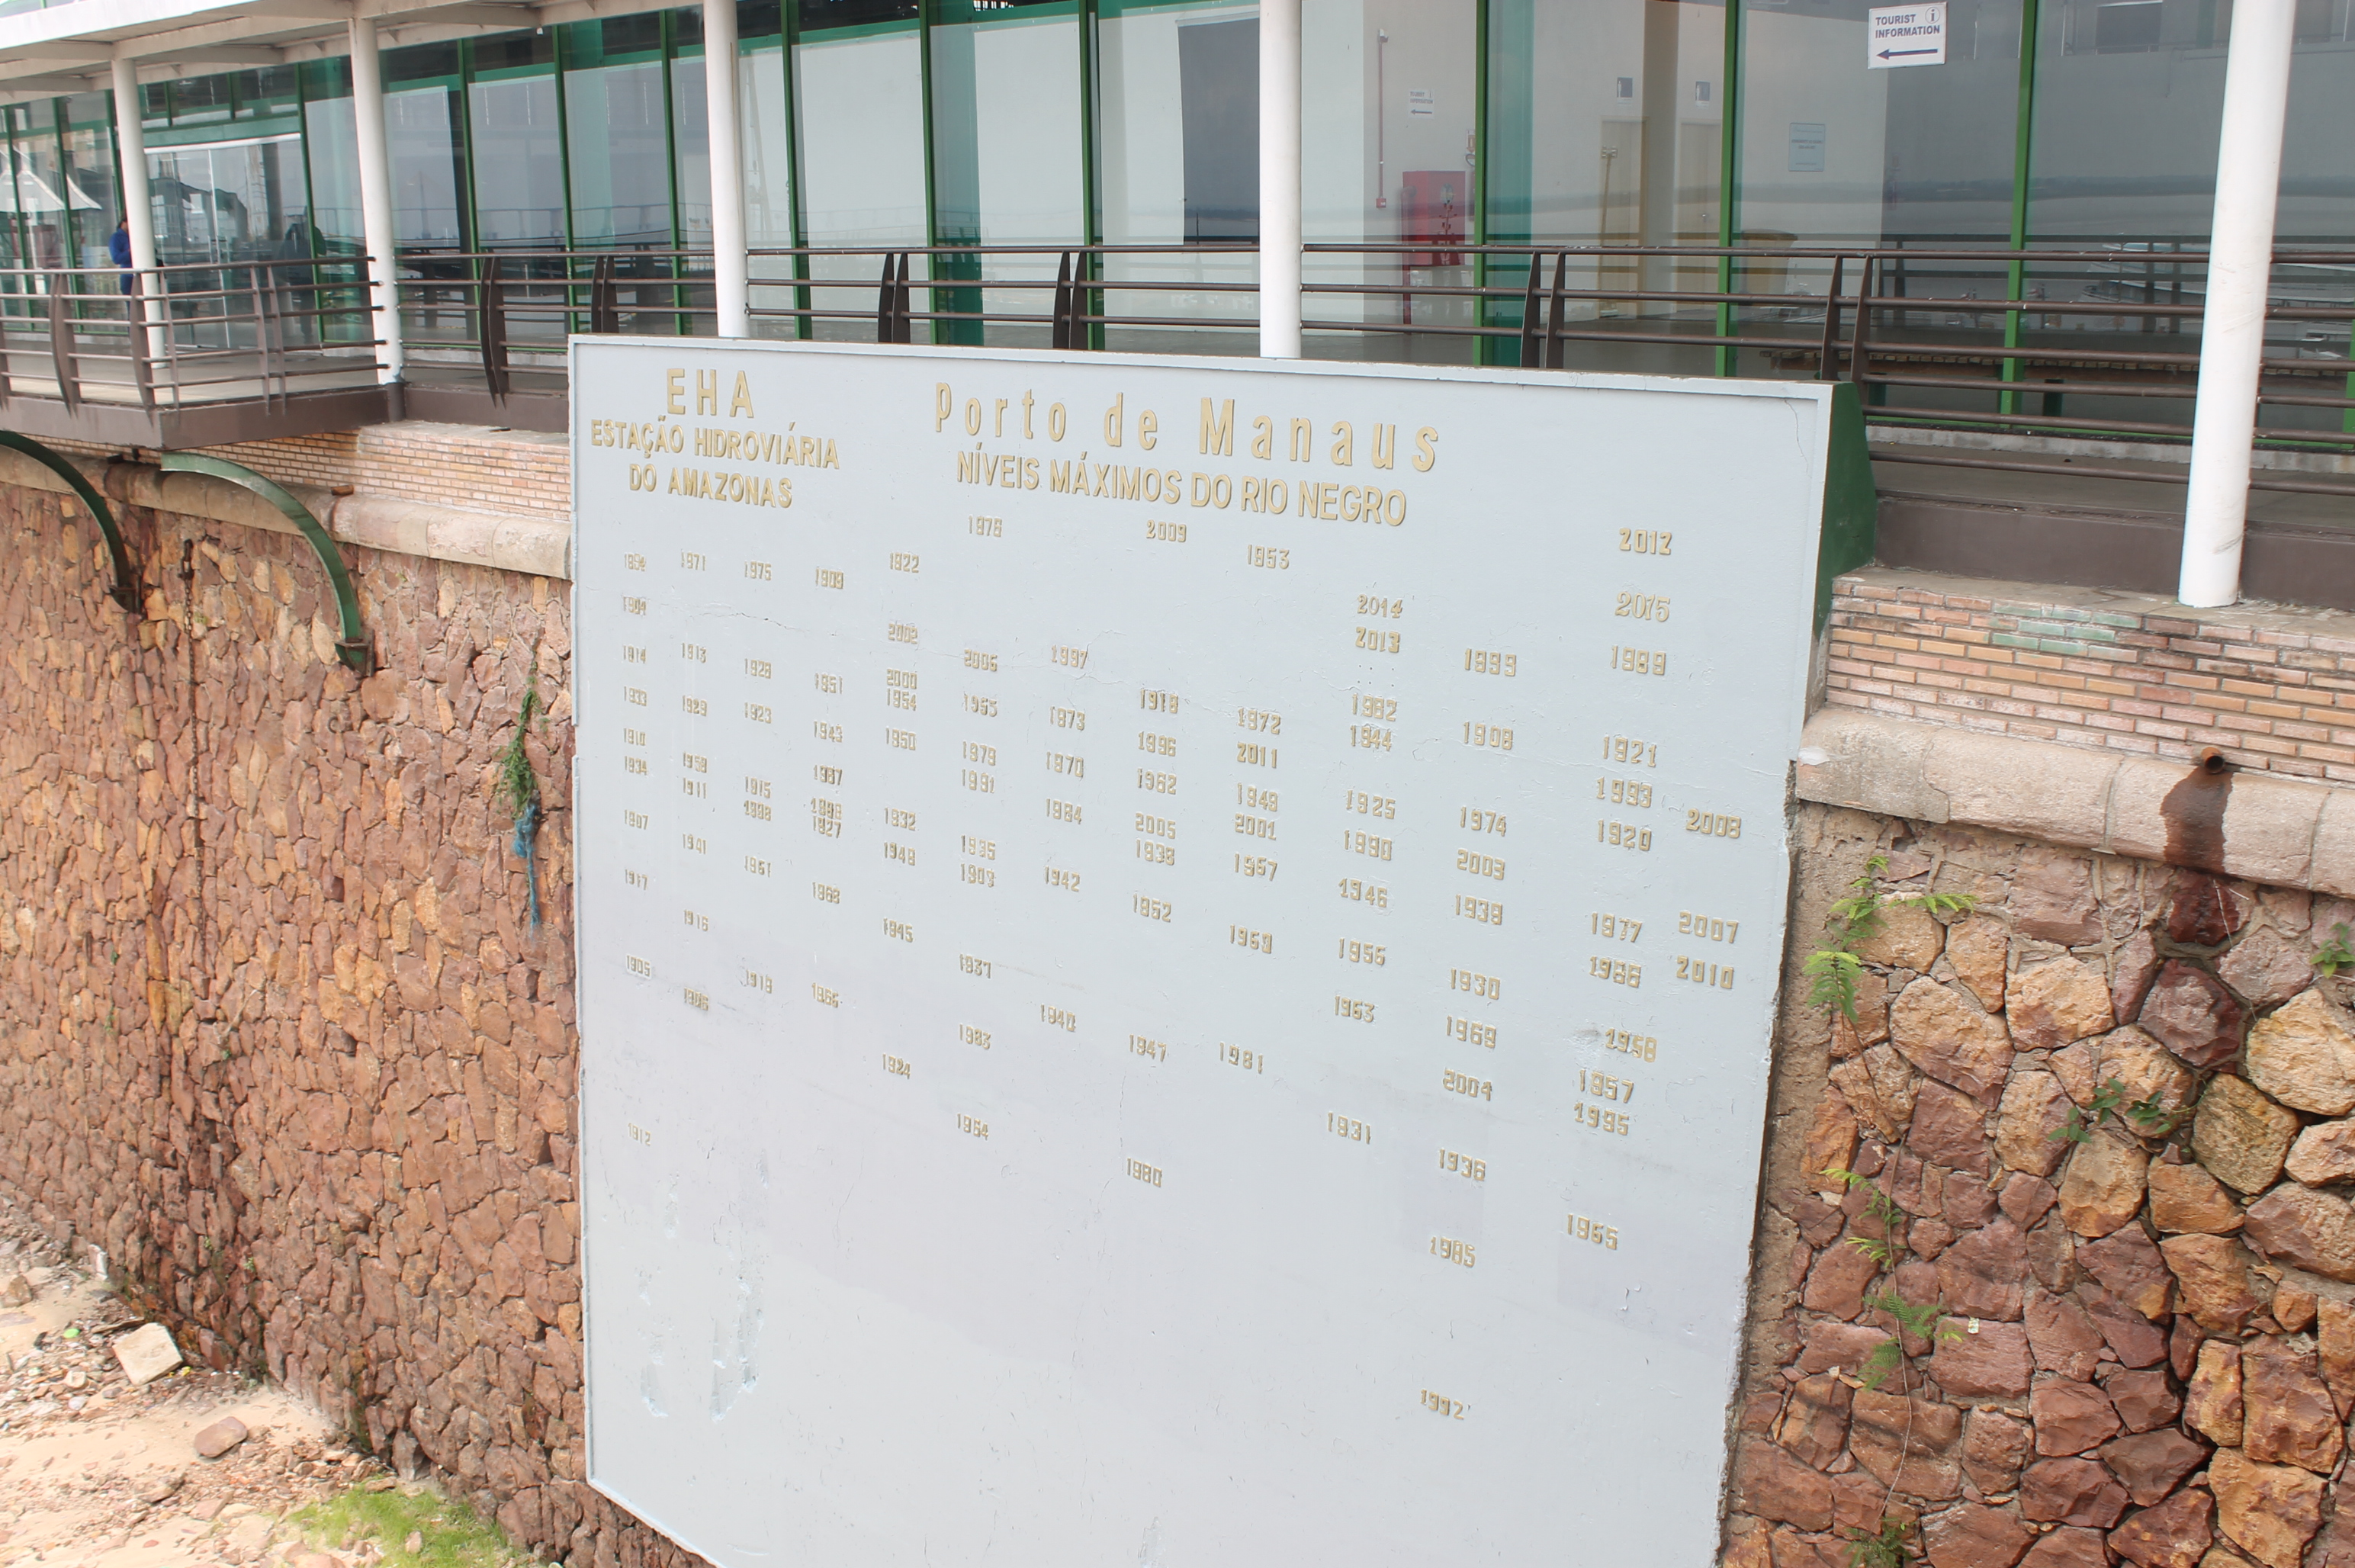
\includegraphics[width=0.6\textwidth]{./img/cota}
\caption{Cota do Rio Negro no Porto de Manaus. Fonte: a pr�pria autora.}
\label{img:cotas}
\end{figure}

O problema da previs�o de dados hidrol�gicos j� foi abordado por diversos trabalhos de Aprendizado de M�quina \cite{Lorrai:RainfallRunoff}, considerando at� mesmo bacias hidrogr�ficas de pequeno porte \cite{Wanderson:Pianco}. No caso da Bacia Amaz�nica, considerando o caso particular do Rio Negro pela sua import�ncia estrat�gica para a cidade de Manaus, os trabalhos que endere�am a previs�o de sua cota e at� mesmo a rela��o desta com a chuva ainda s�o incipientes e mais pesquisas nesta dire��o precisam ser realizadas.


\section{Justificativa} \label{sec:justificativa}
A realiza��o de um projeto de inicia��o cient�fica desta natureza � importante por diversas raz�es. Primeiramente, ressalta-se o \emph{aspecto aplicado da pesquisa}, na qual dados reais do Rio Negro ser�o utilizados para treinar um algoritmo de Aprendizado de M�quina. Os resultados obtidos poder�o ser divulgados junto a especialistas na �rea de Hidrologia, por exemplo, para analisar a viabilidade da sua utiliza��o como refer�ncia na cidade de Manaus. Esta � uma maneira de divulgar o trabalho realizado na institui��o junto � sociedade.

Levando em conta a utiliza��o da Aprendizagem de M�quina, a execu��o deste projeto ir� propiciar ao estudante a possibilidade de \emph{lidar com quest�es da Intelig�ncia Artificial} que incluem, por exemplo, configurar e treinar modelos, comparar resultados obtidos por modelos diferentes, investigar resultados recentes apresentados na literatura, dentre outros.

Outros dos aspectos que ressaltam a relev�ncia da execu��o deste trabalho � a sua \emph{motiva��o pr�tica} e \emph{interdisciplinaridade}. O aluno estar� engajado na resolu��o de uma quest�o pr�tica da cidade em que ele reside, cujos resultados podem vir a ter um impacto positivo para todos os cidad�os. No tocante � interdisciplinaridade, a realiza��o deste projeto ir� favorecer as discuss�es e intera��es com professores, principalmente da �rea de Meteorologia, propiciando uma troca de conhecimentos. Isto � enriquecedor para o discente, pois poder� lidar com conceitos de outras �reas, aplicando m�todos e t�cnicas pr�prios da Computa��o, construindo um espa�o de coopera��o.

A realiza��o deste projeto de inicia��o cient�fica permitir� ao estudante a \emph{viv�ncia de conceitos} de diversas disciplinas, o \emph{desenvolvimento de uma aplica��o pr�tica} de t�cnicas, m�todos e modelos da Aprendizagem de M�quina e ir� ampliar seus horizontes para que possa vislumbrar a possibilidade de seguir \emph{carreira acad�mica} em Computa��o.

Para a docente e proponente deste projeto de inicia��o cient�fica, a possibilidade de consolidar um trabalho desta natureza permitir� o \emph{aprofundamento em uma �rea de pesquisa}, o que contribuir� para a amplia��o do seu escopo de atua��o na �rea de Computa��o e que tamb�m ir� colaborar para fortalecer o grupo de pesquisa da institui��o na qual a docente est� engajada.


\section{Objetivos} \label{sec:objetivos}
O objetivo geral deste trabalho � utilizar redes neurais artificiais para prever a cota do Rio Negro. Para alcan�ar esta meta, alguns objetivos espec�ficos precisam ser contemplados, a citar:

\begin{enumerate}
\item Formular um referencial te�rico sobre Redes Neurais, incluindo seu funcionamento, caracter�sticas, tipos, treinamento e utiliza��o;
\item Montar uma base de dados sobre a cota do Rio Negro;
\item Propor, treinar e testar diferentes redes neurais para prever a cota do Rio Negro;
\item Analisar e avaliar a qualidade das redes neurais para o problema em quest�o.
\end{enumerate}


\section{Metodologia} \label{sec:metodologia}
A metodologia para o desenvolvimento deste projeto de inicia��o cient�fica consiste, inicialmente, no \emph{estudo dos conceitos sobre redes neurais}. Para tanto, o aluno ir� considerar a literatura desta �rea para entender as bases biol�gicas deste modelo computacional, como funcionam, quais as caracter�sticas e os diferentes tipos. Al�m disso, ir� considerar com mais detalhes os aspectos de treinamento destas redes, especialmente considerando o algoritmo \emph{backpropagation} de Levenberg-Marquadt. � importante enfatizar que esta etapa tamb�m contempla o aprendizado da manipula��o de ambientes computacionais ou bibliotecas para lidar com o modelo de computa��o considerado.

O pr�ximo passo do trabalho considerar� a \emph{prepara��o da base de dados} sobre o problema. Nesta etapa, o aluno ir� consultar a literatura e �rg�os especializados para obter dados sobre a cota do Rio Negro e sobre vari�veis meteorol�gicas, relacionando-as de acordo com o per�odo de tempo. Quanto �s vari�veis meteorol�gicas, � poss�vel fazer uso do Banco de Dados Meteorol�gicos para Ensino e Pesquisa (BDMET), mantido pelo Instituto Nacional de Meteorologia (INMET) \cite{INMET:Site}. Para os dados da cota do Rio Negro, a Superintend�ncia Estadual de Navega��o, Portos e Hidrovias poder� ser consultada.

Levando em conta as duas tarefas realizadas previamente, o aluno ir� \emph{treinar e testar as redes neurais} para o problema em quest�o, considerando diferentes arquiteturas para as mesmas. A base de dados ser� utilizada para aprendizado, ficando uma parte da mesma reservada para os testes de predi��o. A sa�da da rede neural ser� um um valor correspondente � cota do Rio Negro prevista para um determinado instante de tempo. Nesta etapa, sempre que poss�vel ser�o consideradas m�tricas sobre o desempenho das redes constru�das.

Em seguida, ser� realizada a \emph{avalia��o dos resultados}. Nesta etapa, m�tricas como erro m�dio quadr�tico e acur�cia ser�o utilizadas para mensurar a adequa��o das referidas redes para o problema em quest�o. Ser� poss�vel, tamb�m, comparar as redes entre si e eleger um subconjunto mais adequado para o referido cen�rio.

Al�m das atividades relatadas, n�o se pode deixar de mencionar a \emph{produ��o dos relat�rios} parcial e final, que s�o essenciais para o andamento do projeto. Esta atividade possuir� um acompanhamento mais minucioso e utilizar� artefatos produzidos ao longo do andamento do projeto para a composi��o destes relat�rios.


\section{Cronograma das Atividades} \label{sec:cronograma}
Uma vis�o geral do cronograma das atividades a serem desenvolvidas ao longo deste projeto podem ser vistas na Tabela \ref{tab:cronograma}. Elas possuem rela��o com as atividades listadas na Se��o \ref{sec:metodologia}, a qual detalha a metodologia que o projeto de pesquisa dever� seguir.


\begin{table}[h!]
\caption{Cronograma de atividades levando em considera��o os doze meses ($08/2014$ a $07/2015$) para a realiza��o do PAIC.} \label{tab:cronograma}
\begin{center}
\begin{small}
\begin{tabular}{p{5cm}ccccccccccccc}
  \toprule
                  &  &  & \textbf{2016}  &  &  &  &  & & \textbf{2017} &  &  & \\
                & \textbf{08} & \textbf{09} & \textbf{10} & \textbf{11} & \textbf{12} & \textbf{01} & \textbf{02} & \textbf{03} & \textbf{04} & \textbf{05} & \textbf{06} & \textbf{07}\\
  \midrule
  \textbf{Estudo dos Conceitos sobre Redes Neurais}     &      X      &   X        &         X   &            &            &            &            &            &             &             &               &      \\
  \textbf{Prepara��o da Base de Dados}                                     &            &      X     &      X     &            &            &            &            &            &             &             &               &      \\
  \textbf{Treinar e Testar as Redes Neurais}                                                &            &            &            &      X     &     X       & X           &      X      &    X        &   X          &             &               &      \\
  \textbf{Avalia��o dos Resultados}                               &            &            &            &            &            &          &            &            &             &      X       &      X         &      \\
  \textbf{Produ��o dos Relat�rios}                                               &            &            &            &            &     X       &           &            &            &             &             &               &   X  \\
  \bottomrule
\end{tabular}
\end{small}
\end{center}
\end{table}



\addcontentsline{toc}{section}{Refer�ncias}
\bibliography{ref}

\appendix

%% M�ximo: 4 p�ginas
%\newpage
%\section{Plano de Atividades do Bolsista} \label{sec:apendice}
%Neste ap�ndice ser� detalhado o plano de atividades do bolsista. Para tanto, na Se��o \ref{sec:objetivosEspecificos} ser�o detalhados os objetivos espec�ficos a serem alcan�ados pelo bolsista; na Se��o \ref{sec:atividades} ser�o detalhadas as atividades a serem cumpridas, as quais devem ser realizadas respeitando os prazos do cronograma da Se��o \ref{sec:cronogramaDetalhado}. Por fim, os aspectos da relev�ncia e interesse do trabalho proposto ser�o apresentados na Se��o \ref{sec:relevancia}.

\subsection{Objetivos Espec�ficos} \label{sec:objetivosEspecificos}

Os objetivos espec�ficos em rela��o a plano de trabalho a ser seguido pelo bolsista s�o:

\begin{enumerate}
\item Efetuar revis�es na literatura sobre as transformadas cl�ssica e qu�ntica de Fourier;
\item Identificar contribui��es existentes sobre a simula��o da transformada qu�ntica de Fourier. Se houver, elencar vantagens, desvantagens e limita��es destes trabalhos existentes;
\item Avaliar a exist�ncia de pacotes, estruturas de dados, linguagens de programa��o e elementos relacionados que possam auxiliar na simula��o da transformada qu�ntica de Fourier em computadores cl�ssicos;
\item Implementar a simula��o da transformada qu�ntica de Fourier utilizando os elementos identificados nas etapas anteriores;
\item Efetuar testes e documentar a implementa��o realizada;
\item Elaborar semin�rios que divulguem o conhecimento adquirido em cada etapa, bem como apresentando o resultado final da simula��o e suas funcionalidades;
\item Redigir os relat�rios parcial e final exigidos pelo Programa de Bolsas de Inicia��o Cient�fica.
\end{enumerate}

\subsection{Atividades} \label{sec:atividades}

O detalhamento das atividades a serem realizadas pelo bolsista est� apresentado abaixo. Algumas delas possuem uma descri��o dos pontos particulares que devem contemplar.

\begin{enumerate}[{\textbf{Atividade }}1{.}]
\item Estudo dirigido sobre a transformada cl�ssica de Fourier. Neste estudo dever�o ser inclu�das a sua formula��o matem�tica, os diferentes algoritmos que podem implement�-la, bem como um levantamento de diferentes �reas nas quais esta transformada � aplicada;
\item Realizar um semin�rio com os resultados obtidos acerca da transformada cl�ssica de Fourier;
\item Estudo dirigido sobre a transformada qu�ntica de Fourier. Este estudo deve incluir as provas de corretude, a resolu��o de exerc�cios, a estima��o dos custos, os gr�ficos que podem ser gerados, e um levantamento de aplica��es desta transformada em diferentes algoritmos qu�nticos;
\item Realizar um semin�rio com os resultados obtidos acerca da transformada qu�ntica de Fourier;
\item Efetuar um levantamento sobre t�cnicas para simula��o de algoritmos qu�nticos em computadores cl�ssicos. Este levantamento deve levar em considera��o aspectos como desempenho, pacotes existentes, estruturas de dados mais adequadas, etc;
\item Efetuar um levantamento, se houver, sobre as iniciativas j� existentes para simula��o da transformada qu�ntica de Fourier. Elencar as caracter�sticas, vantagens, desvantanges e limita��es destas t�cnicas;
\item Iniciar a implementa��o da simula��o da transformada qu�ntica de Fourier em uma linguagem de programa��o escolhida a partir do resultado das atividades anteriores. Priorizar nesta implementa��o a possibilidade de diferentes entradas de dados, mostrar o passo a passo de algumas opera��es e tamb�m apresentar gr�ficos ao final do processo, que ajudem ao usu�rio a compreender o resultado do processamento;
\item Realizar testes na implementa��o constru�da, com o intuito de assegurar a aus�ncia de \emph{bugs}, verificar a adequa��o para os usu�rios, e suportar um certo n�mero de sistemas operacionais diferentes;
\item Documentar a aplica��o para que usu�rios possam utiliz�-la de maneira mais simples e tamb�m para que desenvolvedores possam incluir novas funcionalidades com um esfor�o relativamente pequeno;
\item Fazer um semin�rio apresentando a simula��o da transformada de Fourier, destacando tamb�m as funcionalidades existentes, possibilidades de configura��o, etc.;
\item Disponibilizar a aplica��o em um reposit�rio de software para  que possa ser acessado pela comunidade cient�fica;
\item Redigir relat�rio parcial do PIBIC;
\item Redigir relat�rio final do PIBIC;
\end{enumerate}

\subsection{Cronograma de Execu��o Detalhado} \label{sec:cronogramaDetalhado}

As atividades listadas na se��o anterior ser�o desenvolvidas ao longo dos doze meses do PIBIC de acordo com o cronograma da Tabela \ref{tab:cronogramaDetalhado}.

\begin{table}[h!]
\caption{Tabela contendo a organiza��o das atividades de $1$ a $13$ descritas na Se��o \ref{sec:atividades}, levando em considera��o os doze meses para a realiza��o do PIBIC.} \label{tab:cronogramaDetalhado}
\begin{center}
\begin{tabular}{cccccccccccccc}
  \toprule
                                & \textbf{AGO} & \textbf{SET} & \textbf{OUT} & \textbf{NOV} & \textbf{DEZ} & \textbf{JAN} & \textbf{FEV} & \textbf{MAR} & \textbf{ABR} & \textbf{MAI} & \textbf{JUN} & \textbf{JUL} \\
  \midrule
  \textbf{A1}   &      X     &            &            &            &            &            &            &            &             &             &               &      \\
  \textbf{A2}   &            &    X       &            &            &            &            &            &            &             &             &               &      \\
  \textbf{A3}   &            &    X       &            &            &            &            &            &            &             &             &               &      \\
  \textbf{A4}   &            &            &    X       &            &            &            &            &            &             &             &               &      \\
  \textbf{A5}   &            &            &    X       &    X       &            &            &            &            &             &             &               &      \\
  \textbf{A6}   &            &            &            &    X       &            &            &            &            &             &             &               &      \\
  \textbf{A7}   &            &            &            &            &    X       &    X       &      X     &      X     &    X        &             &               &      \\
  \textbf{A8}   &            &            &            &            &            &            &            &            &    X        &     X       &               &      \\
  \textbf{A9}   &            &            &            &            &            &            &            &            &             &     X       &               &      \\
  \textbf{A10}  &            &            &            &            &            &            &            &            &             &             &       X       &      \\
  \textbf{A11}  &            &            &            &            &            &            &            &            &             &             &       X       &      \\
  \textbf{A12}  &            &            &            &            &     X      &            &            &            &             &             &               &      \\
  \textbf{A13}  &            &            &            &            &            &            &            &            &             &             &               &    X \\
  \bottomrule
\end{tabular}
\end{center}
\end{table}


\subsection{Relev�ncia e Interesse do Trabalho Proposto} \label{sec:relevancia}

O resultado do projeto em quest�o possui contribui��es em diversos aspectos. O primeiro deles � que auxilia na compreens�o da transformada de Fourier em si, o que pode ser �til tamb�m para alunos de outras �reas, a citar Matem�tica, Computa��o, Engenharias, etc. Al�m disso, os relat�rios produzidos ao longo do projeto, bem como os semin�rios, podem servir para embasar a realiza��o de outras pesquisas, a exemplo daquelas que vierem a utilizar o algoritmo da transformada qu�ntica de Fourier como um de seus componentes. Considerando o programa que efetua a simula��o, a primeira contribui��o deste � auxiliar na realiza��o de novas pesquisas e tamb�m na reprodu��o de resultados j� apresentados na literatura, como uma maneira de valid�-los. Por fim, de maneira geral, a realiza��o deste projeto pode consolidar material de apoio no ensino da Computa��o e Comunica��es Qu�nticas, apresentando os passos que comp�em o algoritmo de maneira interativa e com a utiliza��o de gr�ficos.

Em rela��o ao Instituto de Estudos em Computa��o e Informa��o Qu�nticas (IQuanta), sediado na UFCG e no qual o trabalho ser� desenvolvido, a realiza��o de mais um projeto de inicia��o cient�fica � de extrema import�ncia, pois produz uma melhor compreens�o de resultados consolidados na literatura que, apesar disso, possuem um grande n�mero de conceitos envolvidos, especialmente oriundos da Matem�tica. Esta explora��o contribui n�o s� para o aluno que desenvolve o projeto, mas para todo o grupo, que ganha com o conhecimento compartilhado nos semin�rios e relat�rios, e tamb�m com o simulador produzido, que servir� de apoio nas mais diversas pesquisas. Outro aspecto que refor�a a import�ncia da realiza��o desta pesquisa para o instituto � no tocante � forma��o de pessoal, visto que esta � uma �rea multidisciplinar. Quanto mais cedo se d� esta introdu��o, a experi�ncia verificada ao longo do tempo mostra que melhor � o desempenho destes alunos, os quais costumam seguir pela carreira acad�mica na p�s-gradua��o.

Al�m dos benef�cios para a comunidade cient�fica e para o IQuanta, n�o se pode deixar de mencionar as vantagens para o bolsista que ir� desenvolver o projeto em quest�o. O desenvolvimento das habilidades de comunica��o escrita, oral e de programa��o s�o as contribui��es mais diretas na forma��o deste aluno. Vale mencionar que a responsabilidade, o comprometimento e o respeito aos prazos tamb�m s�o outras virtudes adquiridas e desenvolvidas no decorrer do projeto, que ser�o �teis tanto no meio acad�mico como tamb�m no mercado de trabalho. Al�m disso, a viv�ncia em um ambiente acad�mico de uma maneira mais intensa, acompanhando o desenvolvimento de outras pesquisas, assistindo semin�rios de temas diversos, etc. amplia os horizontes desse aluno e faz com que este torne-se mais envolvido e respons�vel pela sua pr�pria forma��o.


\end{document}

